\documentclass[11pt, xcolor={dvipsnames}, hyperref={colorlinks, allcolors=Blue}]{beamer}


% Packages
\usepackage{graphicx}
\usepackage{caption, subcaption}
\usepackage{tikz}
\usepackage{amsmath, amsfonts, amssymb}
\usepackage{booktabs}
\usepackage{apacite}
\usepackage{multirow}
\usepackage{doi}
\usepackage{textpos}
\usepackage{lipsum}
\usepackage{amsfonts, amsmath}
\usepackage{wrapfig}
\usepackage{animate}
\usepackage{cleveref}


\renewcommand\doiprefix{}


\usepackage{tikz}
\usetikzlibrary{shapes, fit}





%%%%%%%%%%%%%%%%%%%%%%%%%%%%%%%%%%%%%%%%%%%%%%
% Custom commands
\newcommand\bc[1]{{\usebeamercolor[fg]{frametitle} {\textbf{#1}}}} % bold and color
\newcommand{\into}{\rightarrow}








%%%%%%%%%%%%%%%%%%%%%%%%%%%%%%%%%%%%%%%%%%%%%%
% Set CSIRO Theme
\usetheme{Boadilla}
\usecolortheme{rose}

%%%%%%%%%%%%%%%%%%%%%%%%%%%%%%%%%%%%%%%%%%%%%%
% Make citation font tiny
\renewcommand{\bibliographytypesize}{\tiny}

%%%%%%%%%%%%%%%%%%%%%%%%%%%%%%%%%%%%%%%%%%%%%%
% Fonts
\usefonttheme{serif} % Serif font
\setbeamertemplate{enumerate items}[default] % Don't use bullets in enumerate.

%%%%%%%%%%%%%%%%%%%%%%%%%%%%%%%%%%%%%%%%%%%%%%%
% Remove navigation bar
\setbeamertemplate{navigation symbols}{}
%%%%%%%%%%%%%%%%%%%%%%%%%%%%%%%%%%%%%%%%%%%%%%


% Frontmatter
\title[ECON 8000 -  Lecture 1]{Lecture 1: Real Analysis}
\author[University of Queensland]{Robert Garrard}
\date[\today]{} 


%%%%%%%%%%%%%%%%%%%%%%%%%%%%%%%

% Common commands
\newcommand{\R}{\mathbb{R}}
\newcommand{\N}{\mathbb{N}}
\newcommand{\Z}{\mathbb{Z}}
\newcommand{\Q}{\mathbb{Q}}
\renewcommand{\P}{\mathbb{P}}
\newcommand{\E}{\mathbb{E}}

\renewcommand{\implies}{\Rightarrow}
\newcommand{\halmos}{\hfill$\blacksquare$}

%%%%%%%%%%%%%%%%%%%%%%%%%%%%%%%%
% Custom environments with counters

\newcounter{Lecture}
\addtocounter{Lecture}{1}

\newcounter{exercise}
\newenvironment{exercise}[1][]{\refstepcounter{exercise}\par\medskip
   \noindent {\bc{Exercise}~\bc{\theLecture.\theexercise} #1}}{\medskip}
%%%%%%%%%%%%%%%%%%%%%%%%%%%%%%%%

% Tikz
\usetikzlibrary{arrows,shapes,trees, positioning}

%%%%%%%%%%%%%%%%%%%%%%%%%%%%%%


\begin{document}

\begin{frame}
\titlepage


\begin{picture}(0,0)
\put(35,-50){\hbox{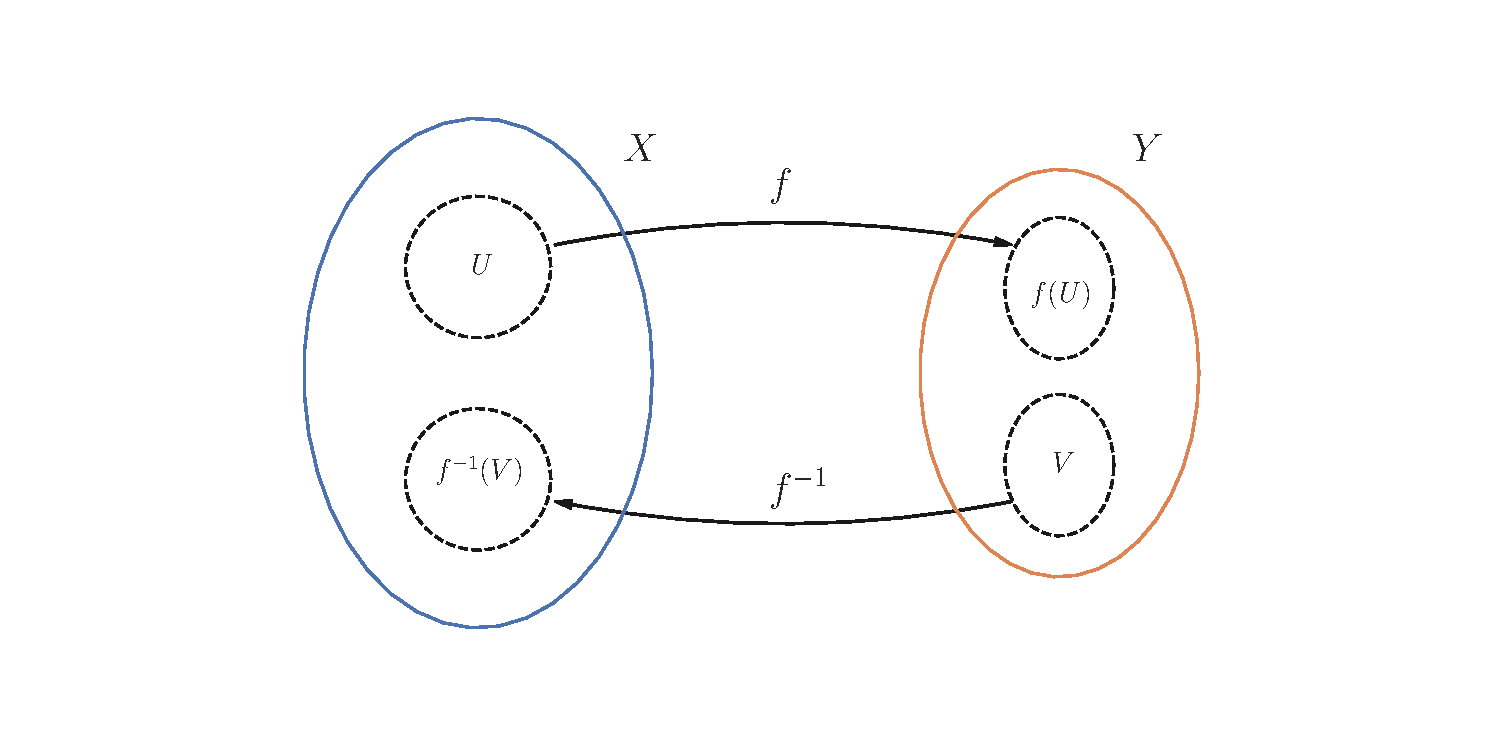
\includegraphics[width=0.8\textwidth, trim={0cm, 1cm, 0cm, 1cm}, clip]{functions.pdf}}}
\end{picture}

\vfill
\end{frame}

%%%%%%%%%%%%%%%%%%%%%%%%%%%%%
\begin{frame}{Housekeeping}

\bc{Contact:}\\

Rob Garrard\\
\href{mailto:r.garrard@uq.edu.au}{r.garrard@uq.edu.au}\\
Consultation: TBD

\bigskip

\bc{Topics Covered:}

Real Analysis, Linear Algebra, Probability and Statistics, Calculus, Optimization, Dynamic Programming.
\bigskip

\bc{Resources:}

\textit{Mathematics for Economists}. Carl P. Simon \& Lawrence Blume.\\

\textit{Econometric Analysis}. William H. Greene.

\textit{Recursive Methods in Economic Dynamics}. Robert E. Lucas, Nancy Stokey, with Edward C. Prescott.




\end{frame}


%%%%%%%%%%%%%%%%%%%%%%%%%%%%%
\begin{frame}{Housekeeping}


\bc{Assessment}:
\begin{itemize}
	\item Tutorial problems (20\%)
	\begin{itemize}
		\item  Either submitted to Blackboard or handed in at beginning of tutorial starting Week 2.
		\item Problem set covers the Thursday lecture from previous week and Monday lecture from current week.
		\item Can be handwritten or typed at your preference. Please consider using \LaTeX \ (\href{https://www.overleaf.com/}{overleaf.com}).
	\end{itemize}

	\item Take-home assessment \#1 (30\%)
	\begin{itemize}
		\item Due by end of day 25\textsuperscript{th} February.
		\item Covers first 5 lectures.
	\end{itemize}
	

	\item Take-home assessment \#2 (50\%)
	\begin{itemize}
		\item Due by end of day Wednesday 25\textsuperscript{th} March.
		\item Covers entire course.
	\end{itemize}
\end{itemize}

\end{frame}
%%%%%%%%%%%%%%%%%%%%%%%%%%%%%


\begin{frame}{Vocabulary: Sets}

A \bc{set} is an unordered collection of objects. 

\begin{center}
	\begin{tabular}{p{3cm} p{3cm} p{3cm}}
$A = \{0, 1\}$  & $B = \{0, \{1\}\}$  & $\emptyset = \{\}$
\end{tabular}
\end{center}
\bigskip

Membership is denoted with `$\in$', non-membership with `$\not\in$'.
\begin{center}
	\begin{tabular}{p{3cm} p{3cm} p{3cm}}
		$0 \in A$ & $\{1\} \in B$ & $0 \not\in C$
	\end{tabular}
\end{center}
\bigskip

Repeated elements aren't counted seperately: $\{0, 1, 1\} = \{0, 1\}$
\bigskip

Some common sets:

\begin{center}
\setlength{\tabcolsep}{.5cm}
\renewcommand{\arraystretch}{1.2}
	\begin{tabular}{l l}
	$\N = \{1, 2, 3, 4, \dots\}$ & $\Z = \{0, 1, -1, 2, -2, \dots\}$\\
	$\Q = \{ \frac{a}{b} \ | \ a, b \in \Z\}$ & $\mathbb{C} = \{a + bi \ | \ i = \sqrt{-1}; a,b \in \R\}$
	\end{tabular}
\end{center}

\end{frame}

%%%%%%%%%%%%%%%%%%%%%%%%%%%%%

\begin{frame}{Vocabulary: Logical Statements}

A logical \bc{proposition} is a statement that can be either True or False.

\begin{center}
	\begin{tabular}{l}
	$P$: It rained today.\\
	$Q: \sqrt{2} \in \Q$
	\end{tabular}
\end{center}

We can transform and combine propositions using \bc{logical operators}.
\medskip 

\begin{center}
\setlength\tabcolsep{.5cm}
\begin{tabular}{l|l|l}
Operator & Notation& Meaning\\\toprule
Negation & $\neg$ p& not p\\
Conjunction & $p \wedge q$ & p and q \\
Disjunction & $p \vee q$ & p or q (or both)\\
Implication & $p \implies q$ & p implies q/if p then q\\
Biconditional & $p \iff q$ & p if and only if q
\end{tabular}
\end{center}

\end{frame}

%%%%%%%%%%%%%%%%%%%%%%%%%%%%%

\begin{frame}{Vocabulary: Logical Statements}

We can determine under what circumstances a compound proposition is true or false using a \bc{truth table}.

\begin{table}	
	\centering
	\begin{subtable}{0.3\textwidth}
	\caption*{Negation}
	\centering
	\begin{tabular}{l | l}
		$p$ & $\neg p$\\\toprule
		0 & 1\\
		1 & 0\\
		\multicolumn{2}{l}{}\\ % Blank rows for spacing
		\multicolumn{2}{l}{}\\
	\end{tabular}
	\end{subtable}
	\begin{subtable}{0.3\textwidth}
	\caption*{Conjunction}
	\centering
	\begin{tabular}{l | l | c}
		$p$ & $q$ & $p \wedge q$\\\toprule
		0 & 0 & 0\\
		0 & 1 & 0\\
		1 & 0 & 0\\
		1 & 1 & 1\\
	\end{tabular}
	\end{subtable}
	\begin{subtable}{0.3\textwidth}
	\caption*{Disjunction}
	\centering
	\begin{tabular}{l | l | c}
		$p$ & $q$ & $p \vee q$\\\toprule
		0 & 0 & 0\\
		0 & 1 & 1\\
		1 & 0 & 1\\
		1 & 1 & 1\\
	\end{tabular}
	\end{subtable}
	\newline
	
	\begin{subtable}{0.3\textwidth}
	\caption*{Implication}
	\centering
	\begin{tabular}{l | l | c}
		$p$ & $q$ & $p \implies q$\\\toprule
		0 & 0 & 1\\
		0 & 1 & 1\\
		1 & 0 & 0\\
		1 & 1 & 1\\
	\end{tabular}
	\end{subtable}
		\begin{subtable}{0.3\textwidth}
	\caption*{Biconditional}
	\centering
	\begin{tabular}{l | l | c}
		$p$ & $q$ & $p \iff q$\\\toprule
		0 & 0 & 1\\
		0 & 1 & 0\\
		1 & 0 & 0\\
		1 & 1 & 1\\
	\end{tabular}
	\end{subtable}
	
\end{table}

\end{frame}

%%%%%%%%%%%%%%%%%%%%%%%%%%%%%%%
\begin{frame}{Vocabulary: Logical Statements}

\begin{exercise}

Let $x \in \Z$. What is the truth value of the following propositions?

\begin{enumerate}
	\item $x \geq 0 \vee x < 0$

	\item $x^{2} > 0 \implies x > 0$

	\item $x^{2} \text{ is even} \iff x \text{ is even}$

	\item $x \text{ is prime} \wedge x \text{ is even} \implies x = 2$

	\item {[Harder]} $x^{2} = 2 \implies x = 10$
\end{enumerate}

\end{exercise}
\end{frame}

%%%%%%%%%%%%%%%%%%%%%%%%%%%%%%%
\begin{frame}{Vocabulary: Logical Statements}

Propositions that are: always true are called \bc{tautologies}; always false are called \bc{contradictions}; sometimes true, sometimes false are called \bc{contingent} statements.
\bigskip

\begin{exercise}
\begin{enumerate}
	\item Show that $p \wedge \neg p$ is a contradiction.
	\item Show that $ p \implies q \iff \neg q \implies \neg p$ is a tautology.
\end{enumerate}
\end{exercise}
\vfill
\end{frame}


%%%%%%%%%%%%%%%%%%%%%%%%%%%%%%%
\begin{frame}{Vocabulary: Logical Statements}

We may want some propositions to refer only to a particular set of quantities. Some common \bc{quantifiers} are:
\begin{center}
\begin{tabular}{l|l|l}
Quantifier & Notation& Meaning\\\toprule
Universal quantifier & $\forall$ &`for all' or `for every'\\
Existential quantifier & $\exists$ & `there exists'
\end{tabular}
\end{center}
\medskip

\begin{block}{Example}

Write the following statements in logical notation.

\begin{enumerate}
	\item ``Every natural number is greater than zero''.\\
	\ $\forall n \in \N \ n > 0$

	\item ``There is a largest integer''.\\
	\ $\exists N \in \Z \text{ such that } \forall n \in \Z \ \ n \leq N$
\end{enumerate}

\end{block}



 




\end{frame}
%%%%%%%%%%%%%%%%%%%%%%%%%%%%%

\begin{frame}{Vocabulary: Sets}

We can construct new sets out of old with logical operations:


\begin{center}
\begin{tabular}{l|l}
Operator       & Notation\\\toprule
Intersection  & $A \cap B = \{x \in A \wedge x \in B\}$ \\
Union              & $A \cup B = \{x \in A \vee x \in B\} $ \\
Relative Complement & $A\backslash B = \{x\in A \wedge x \not\in B\}$\\
Cardinality & $|A| = \{\text{number of elements in } A\}$
\end{tabular}
\end{center}

When we have a particular universal set $U$ in mind, we can define an absolute complement: $A^{c} = U\backslash A$.
\bigskip

We can talk about a set being contained in another set with a proposition:

$A \subseteq B$ (eqv. $B \supseteq A$) if $\forall a \in A, \ a \in B$.\\
$A \subset B$ (eqv. $B \supset A$) if $\forall a \in A, \ a \in B \wedge \exists b \in B \text{ s.t. } b \not\in A$.\\
\bigskip

And define the \bc{power set} of a set: $\mathcal{P}(A) = \{B \ | \ B \subset A\}$.


\end{frame}
%%%%%%%%%%%%%%%%%%%%%%%%%%%%%

\begin{frame}{Vocabulary: Sets}

\begin{exercise}
	\[A = \{-1, 0, 1\} \qquad B = \N \qquad C = \{a, b\}\]

\begin{enumerate}
	\item $A \cap B$ 
	\item $A \cup B$
	\item $B \cap C$
	\item $A \subset B$ 
	\item $\mathcal{P}(C)$
\end{enumerate}
\end{exercise}
\end{frame}


%%%%%%%%%%%%%%%%%%%%%%%%%%%%%

\begin{frame}{Proof}

\bc{Proof} is argumentation we use to establish the truth or falsehood of a proposition.
\bigskip

Common methods of proof:
\begin{itemize}
	\item \bc{Direct Proof}
		\begin{itemize}
			\item Deductive reasoning, often by syllogism. E.g.,  $p \wedge q \implies r$; $p$ and $q$ are true, therefore $r$ is true.
		\end{itemize}
	\item \bc{Proof by Contraposition}
		\begin{itemize}
			\item Transform a proposition ($p \implies q$) into its contrapositive ($\neg q \implies \neg p$), then use direct proof.
		\end{itemize}
	\item \bc{Proof by Contradiction}
		\begin{itemize}
			\item If $p$ is true, $p \wedge q \implies r$, and $r$ is false; then $q$ must be false.
		\end{itemize}
	\item \bc{Proof by Induction}
		\begin{itemize}
			\item We'll explore this in more detail.
		\end{itemize}
	\item \bc{Proof by Counter-example}
	\begin{itemize}
			\item To prove that a proposition is false, produce an example where it fails.
		\end{itemize}
\end{itemize}

\end{frame}


%%%%%%%%%%%%%%%%%%%%%%%%%%%%%

\begin{frame}{Proof}
\begin{theorem}[De Morgan's Laws]
Let $A$ and $B$ be sets.
	\begin{align*}
		(A \cup B)^{c} = A^{c} \cap B^{c}\\
		(A \cap B)^{c} = A^{c} \cup B^{c}
	\end{align*}
\end{theorem}


\begin{exercise}
\begin{enumerate}
	\item Prove directly the first of De Morgan's laws.
	\item Prove by contraposition that if $x^{2}$ is even, then $x$ is even, $x \in \Z$.
\end{enumerate}
\end{exercise}

\vfill

\end{frame}

%%%%%%%%%%%%%%%%%%%%%%%%%%%%%

\begin{frame}{Proof by Induction}

\bc{Proof by induction} is a convenient method availble to us when the proposition can be split into cases indexed by the natural numbers, $P(n)$, $n\in N$.
\bigskip

To establish the truth of the proposition for each $n$, we must prove:\\

\bc{Base case:} $P(1)$ is true.\\

\bc{Induction step:} $P(n) \implies P(n+1)$.


\end{frame}

%%%%%%%%%%%%%%%%%%%%%%%%%%%%%

\begin{frame}{Proof by Induction}

\begin{block}{Example}
Prove that the sum of the first $n$ integers is: $1 + 2 + 3 + \dots + n = \frac{n(n+1)}{2}$.
\bigskip

\underline{Base case:}\\
Sum of first 1 integers = 1.\\
$\frac{1(1+1)}{2} = \frac{2}{2} = 1$.\\

\bigskip

\underline{Induction step:}\\
 Assume true for the $n^{th}$ case, show true for the $(n+1)^{th}$ case.\\
\bigskip

$(n+1)^{th}$ case is:\\

$1 + 2 + 3 + \dots + n + (n+1) = \frac{n(n+1)}{2} + (n+1) = \frac{n(n+1)}{2} + \frac{2(n+1)}{2}$\\

$ = \frac{(n+1)(n+1 + 1)}{2} $

\halmos

\end{block}


\end{frame}


%%%%%%%%%%%%%%%%%%%%%%%%%%%%%

\begin{frame}{Proof by Induction}
\begin{exercise}
Let $A$ be a finite set. Prove that $|\mathcal{P}(A)| = 2^{|A|}$.\hfill\bigskip
\end{exercise}

\vfill\vfill\vfill
\end{frame}


%%%%%%%%%%%%%%%%%%%%%%%%%%%%%%%%%
%%%%%%%%%%%%%%%%%%%%%%%%%%%%%%%%%

%%%%%%%%%%%%%%%%%%%%%%%%%%%%%
\begin{frame}{The Real Numbers}

\begin{center}
	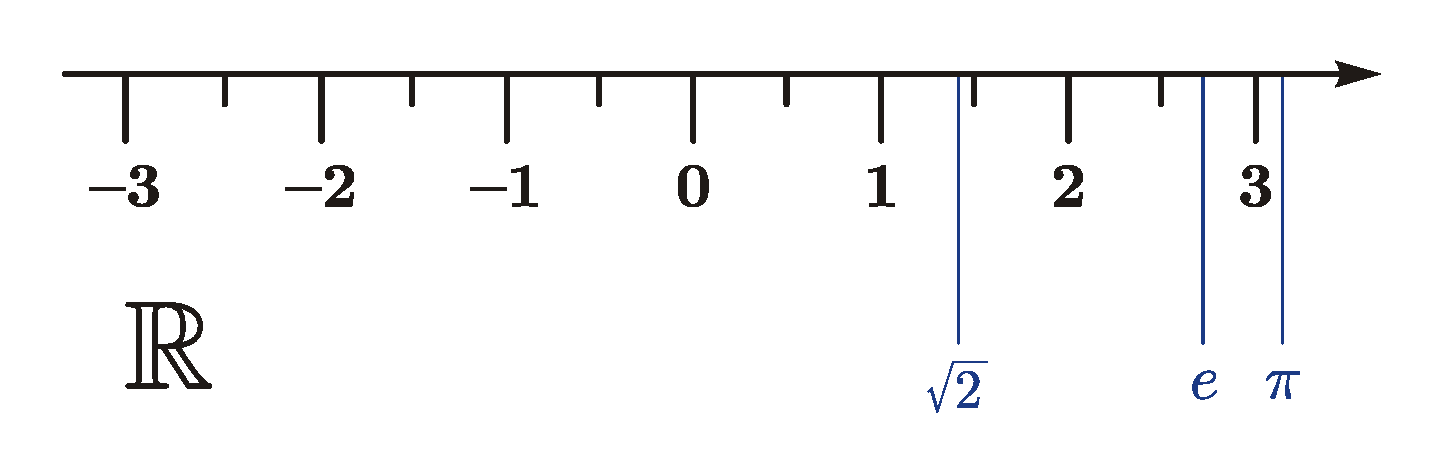
\includegraphics[height=0.75in]{Real_number_line.pdf}
\end{center}

The set of real numbers, $\R$, is the `real' in `real analysis'.\bigskip

Won't get a rigorous treatment here, since we want to get to the useful results from real analysis in the next lecture. We may briefly return to touch on the definition of the real numbers once we've covered Cauchy sequences and completeness, time permitting.\bigskip

We'll need an important feature of the reals:\\
Recall that a subset of numbers, $X$, is \bc{bounded above} if $\exists B$ s.t. $\forall x \in X \ \ x \leq B$.\bigskip

E.g., the interval $(0, 1)$ is bounded above by 2.

\end{frame}

%%%%%%%%%%%%%%%%%%%%%%%%%%%%%%%%
\begin{frame}{The Real Numbers}

\bc{Least Upper Bound property}: Any non-empty subset of the reals that is bounded above has a \emph{least} upper bound. \bigskip

The interval $(0, 1)$ has many upper bounds. $2, 3, \pi$, etc. However, 1 is the unique LUB. \bigskip

Analogously, subsets of real numbers bounded \emph{below} have a \bc{greatest lower bound}.\bigskip

We call the least upper bound of a set the \bc{supremum}, denoted $\sup$.\\
We call the greatest lower bound of a set the \bc{infimum}, denoted $\inf$.\\\bigskip


\textbf{This is not true for the rationals}, $\Q$.\bigskip

\end{frame}
%%%%%%%%%%%%%%%%%%%%%%%%%%%%%%%%%

\begin{frame}{The Real Numbers}
\begin{exercise}
\begin{enumerate}%
	\item Show that the set $\{x \in \Q \ | \ x^{2} < 2\}$ has no supremum.
	\item What are the $\sup$ and $\inf$ of $\{x \in \R \ | \ x^{2} < 2\}$. 
	\item What are the $\sup$ and $\inf$ of bounded intervals in $\R$?
\end{enumerate}
\end{exercise}

\vfill\vfill
\end{frame}

%%%%%%%%%%%%%%%%%%%%%%%%%%%%%%%%
\begin{frame}{Cartesian Product}

The \bc{Cartesian Product} of two sets, $A$ and $B$, is the set of all ordered pairs formed by taking the first element of the pair from $A$ and the second element of the pair from $B$:

\[ A \times B = \{(a,b) \ | \ a \in A, b \in B\} \]

\begin{block}{Example}
\centering
$A = \{1, 2\} \quad \quad B = \{1, 2, 3\}$\\\smallskip
$A \times B = \{(1,1), (1,2), (1,3), (2,1), (2,2), (2,3)\}$
\end{block}

\bigskip

\noindent
The Cartesian product of $n$ sets is the set of all $n$-tuples formed in the same fashion as above. 

\[ \R^{n} = \underbrace{\R \times \R \times \dots \times \R}_{n} = \{(x_{1}, x_{2},...,x_{n}) \ | \ x_{i} \in \R\} \]\\

\end{frame}


%%%%%%%%%%%%%%%%%%%%%%%%%%%%%
\begin{frame}{Binary Relations}

A \bc{binary relation}, $(X, Y, G)$ is an ordered triple where the set $X$ is called the domain, the set $Y$ is called the codomain, and the set G, called the graph, is a subset of the cartesian product of these sets, $G \subseteq X\times Y$.
\bigskip

The graph is a set of ordered pairs, $G = \{(x,y) \ | \ x \in X, y \in Y\}$. If the pair $(x,y) \in G$, we often write $xRy$ and say ``$x$ relates to $y$''. 
\bigskip

\begin{block}{Example}
\begin{enumerate}
\item Let $X = \{1,2,3\}$ and $Y = \{a, b, c\}$. Define the relation $(X,Y,G)$ such that
\[G = \{(1,a), (1,b), (1,c), (2,a), (3, c)\}\]

\item Define the unit circle to be the relation $(\R, \R, G)$ such that
\[G = \{(x,y) \in \R^{2} \ | \ x^{2} + y^{2} = 1\}\]
\end{enumerate}
\end{block}


\end{frame}

%%%%%%%%%%%%%%%%%%%%%%%%%%%%%
\begin{frame}{Economic Application: Preference relations}
\label{slide:PreferenceRelation1}
Consider a set of bundles $X = \{\text{Apples}, \text{Bananas}, \text{Carrots}\}$. \\\bigskip

Our economic agent likes carrots more than apples, and likes apples and bananas equally.\\\bigskip

We can represent these \bc{preferences} with a binary relation from $X$ to itself, $(X, X, \succsim)$, where:

\begin{align*}
\succsim = \{&\text{(Apples, Apples), (Apples, Bananas),  (Bananas, Bananas),}\\
	        & \text{(Bananas, Apples), (Carrots, Carrots), (Carrots, Apples),}\\
		& \text{(Carrots, Bananas)}\}
\end{align*}

We call $\succsim$ the ``weak preference'' relation. \\ \bigskip

Representing preferences as a binary relation is very general. We'll need to place some additional structure on these relations to conform with how we expect real-world preferences to behave.


\end{frame}



%%%%%%%%%%%%%%%%%%%%%%%%%%%%

\begin{frame}{Properties of Relations}

When the domain and codomain of a relation are the same set, the relation \emph{may} exhibit some interesting properties.\bigskip


\begin{block}{Properties of Relations}
\begin{itemize}
\item[] \bc{Reflexive} if \ \ $\forall x\in X \ \ xRx $
\item[] \bc{Irreflexive} if \ $\forall x \in X \ \ \neg xRx$ 
\item[] \bc{Symmetric} if \ $xRy \implies yRx \ \ \forall x,y\in X$
\item[] \bc{Anti-symmetric} if \ $xRy \wedge  yRx \implies x = y\ \ \forall x,y\in X$
\item[] \bc{Asymmetric} if \ $xRy \implies \neg yRx \ \ \forall x,y\in X$
\item[] \bc{Transitive} if \ $xRy \wedge yRz \implies xRz \ \ \forall x,y,z \in X$
\item[] \bc{Weakly Connected} if \ $xRy \vee yRx \ \ \forall x\not = y \in X$
\item[] \bc{Complete} if reflexive and weakly connected.
\end{itemize}
\end{block}

\end{frame}


%%%%%%%%%%%%%%%%%%%%%%%%%%%%%%
\begin{frame}{Properties of Relations}
\begin{exercise}
\begin{enumerate}
	\item Recall the unit circle relation above. Is this relation reflexive, irreflexive, symmetric or transitive?
	\item Show that if a relation is asymmetric, then it is irreflexive.
	\item Consider the game Rock-Paper-Scissors. Let $R$ be the relation ``beats''. Which properties does RPS satisfy?
	\item Which of the properties would the weak preference relation, $\succsim$, satisfy? Verify that they are satisfied for the preferences on slide \ref{slide:PreferenceRelation1}.
\end{enumerate}
\end{exercise}
\end{frame}

%%%%%%%%%%%%%%%%%%%%%%%%%%%%%%

\begin{frame}{Economic Application: Preference relations}
\label{slide:PreferenceRelation2}

A weak preference relation, $\succsim$, is defined to be \bc{rational} if it is \bc{complete} and \bc{transitive}.\bigskip

A rational weak preference relation induces two other useful relations:

\begin{table}
\centering
	\begin{tabular}{l | l | l}
	Name & Symbol & Meaning\\\toprule
	Strict Preference & $x \succ y$ & $x \succsim y \ \wedge \neg \ y \succsim x$\\
	Indifference & $x \sim y$ & $ x \succsim y \ \wedge y \succsim x$\\
	\bottomrule
	\end{tabular}
\end{table}



\end{frame}


%%%%%%%%%%%%%%%%%%%%%%%%%%%%%
\begin{frame}{Functions}

A \bc{function}, $f$, is a binary relation, $(X, Y, G)$, such that:\\

\begin{center}
	\begin{enumerate}
		\item $\forall x \in X \ \exists y \in Y \ s.t \ (x,y) \in f$
		\item $(x,y)\in G \wedge (x,z) \in G \implies y = z$
	\end{enumerate} 
\end{center}

That is, each element in the domain \emph{must} be mapped to \emph{exactly} one object in the codomain.\\\bigskip

Functions (or mappings) are usually written as $f:X\into Y$, where $f$ is the name of the function, $X$ is its domain and $Y$ is its codomain; along with a ``rule'' for assigning each element in $X$ to an element in $Y$.

\end{frame}

%%%%%%%%%%%%%%%%%%%%%%%%%%%%%%
\begin{frame}{Functions}

\begin{block}{Example}
The following are functions:
\begin{itemize}
	\item $f:\R \into \R \quad f(x) = x^{2}$
	\item $\pi:\N\into\N\cup\{0\} \quad \pi(x) = \#\text{ primes} \leq x$.
	\item $g:\{1, 2, 3\}\into\{a, b\} \quad G = \{(1, a), (2, a), (3, a)\}$.
\end{itemize}
\end{block}
\bigskip

\begin{exercise}

Which of the following are functions?
\begin{enumerate}
	\item $f(x) = \frac{1}{x}$
	\item $f:\R\into\R \quad f(x) = \frac{1}{x}$
	\item $g:\R\into\R \quad G = \{(x,y) \in \R^{2} \ | \ x^{2} + y^{2} = 1\}$
	\item The weak preference relation on slide \ref{slide:PreferenceRelation1}
	\item $\P:\mathcal{P}(\{H, T\})\into [0, 1]$ where\\
	$ \P(\{H\}) = \frac{1}{2}, \ \P(\{T\}) = \frac{1}{2}, \ \P(\emptyset) = 0, \ \P(\{H, T\}) = 1$.
\end{enumerate}
\end{exercise}

\end{frame}



%%%%%%%%%%%%%%%%%%%%%%%%%%%%%
\begin{frame}{Properties of Functions}

The \bc{image} of a set $A$ under a function $f$ is the set

\[ f(A) = \{ y \in Y \ | \ \exists x \in A \text{ s.t. } f(x) = y\}\]


The \bc{pre-image} of a set $B$ under a function $f$ is the set
\[ f^{-1}(B) = \{x \in X \ | \ f(x) \in B\} \]

The \bc{range} of a function, $im(f)$,  is the image of its domain.



\begin{block}{Example}
Consider the function $f:\R \into \R$, $f(x) = 2$, and the sets $A = \{1, 2 , 3\}$, $B = \{5, 6\}$, $C = \{2\}$

\begin{align*}
&f(A) = \{2\}&  &f^{-1}(B) = \emptyset&   & f^{-1}(C) = \R&
\end{align*}

\end{block}
\end{frame}

%%%%%%%%%%%%%%%%%%%%%%%%%%%%%
\begin{frame}{Properties of Functions}

\begin{figure}[t]
	\centering
	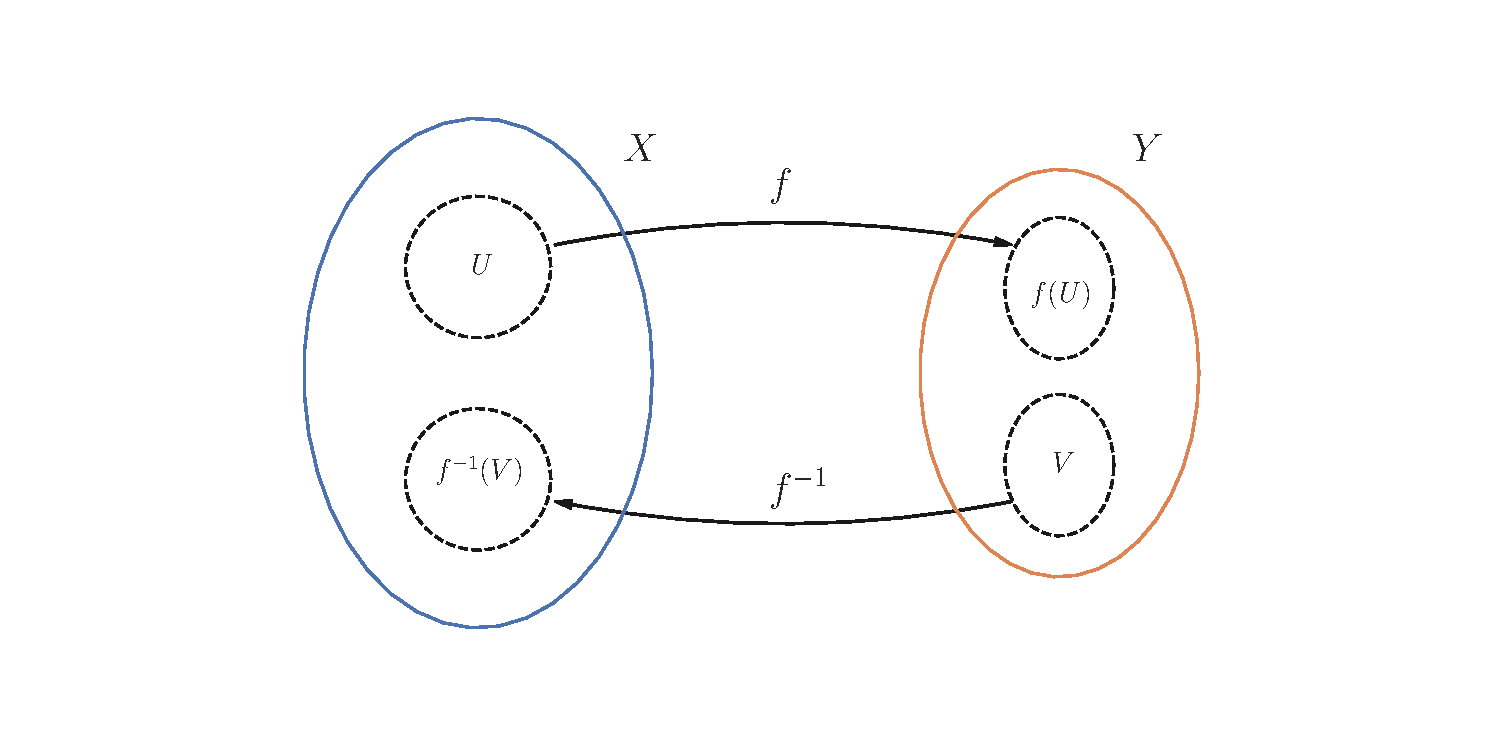
\includegraphics[width=0.8\textwidth]{functions.pdf}
\end{figure}

\begin{exercise}
Let $f:X\to Y$ be a function. Let $U \subseteq X$ and $V \subseteq Y$. Show that
\begin{enumerate}
	\item $U \subseteq f^{-1}(f(U))$.
	\item $f(f^{-1}(V)) \subseteq V$.
\end{enumerate}
\end{exercise}

\end{frame}


%%%%%%%%%%%%%%%%%%%%%%%%%%%%
\begin{frame}{Properties of Functions}

A function $f:X\into Y$ is said to be an 
\begin{itemize}
\item[] \bc{Injection} (one-to-one) if \ $f(a) = f(b) \implies a = b \ \ \forall a,b \in X$
\item[] \bc{Surjection} (onto) if \ $\forall y\in Y \ \exists x \in X \ s.t \ f(x) = y$
\item[] \bc{Bijection} if it is both injective and surjective
\end{itemize}

\bigskip

\begin{block}{Example}
$f:\R \to \R$, $f(x) = x^{2}$ is neither an injection ($-x$ and $x$ both map to the same thing) or surjection (nothing maps to -1).\medskip

$f:\R_{+} \to\R_{+}$, $f(x) = x^{2}$, is a bijection. \medskip


\end{block}

\end{frame}

%%%%%%%%%%%%%%%%%%%%%%%%%%%%%
\begin{frame}{Properties of Functions}
Functions that are bijective possess an \bc{inverse function}, denoted $f^{-1}$.\bigskip

A continuous function $f:\R\to \R$, is invertible iff it is strictly increasing everywhere or strictly decreasing everywhere. If the function is differentiable, it is sufficient to show that $\forall x$, $f^{'}(x) > 0$  or $f^{'}(x) < 0$.

\end{frame}
%%%%%%%%%%%%%%%%%%%%%%%%%%%%


\begin{frame}{Economic Application: A Utility Representation Theorem}

A weak preference relation can be \bc{represented} by a \bc{utility function} if there exists a function $U$ such that

\[ x \succsim y \iff  U(x) \geq U(y)\]

\begin{theorem}
Let $X$ be a finite set and $(X, X, \succsim)$ be a weak preference relation.\\

 The preferences can be represented by a utility function if and only if they are complete and transitive.
\end{theorem}

\end{frame}

%%%%%%%%%%%%%%%%%%%%%%%%%%%%
\begin{frame}{Cardinality, Revisited}

How do we assign cardinality to sets with infinitely many elements, like $\N$, $\Q$, and $\R$?\bigskip


$|A| = |B|$ iff there exists a bijection, $f:A\into B$.\bigskip

Defining cardinality in this way, we see that not all infinities are equal. In particular, $|\N| \not= |\R|$. (see \href{https://en.wikipedia.org/wiki/Cantor\%27s\_diagonal_argument}{Cantor's Diagonal Argument})\bigskip

We refer to sets whose cardinality is either finite or equal to $|\N|$ as having \bc{countably} many elements. Set's that do not satisfy this criterion, such as $\R$, have \bc{uncountably} many elements.

\end{frame}

\begin{frame}{Cardinality, Revisited}

\begin{exercise}
\begin{enumerate}
	\item Show that the set of non-negative even numbers $E = \{0, 2, 4, 6, \dots\}$ has the same cardinality as the naturals.
	\item Show that the interval $(0, 1)$ has the same cardinality as the interval $(0, a)$, $a>0$.
\end{enumerate}
\end{exercise}
\end{frame}
%%%%%%%%%%%%%%%%%%%%%%%%%%%%%
\begin{frame}{Metric Spaces}

A \bc{space} is just a set endowed with some sort of structure.\\\bigskip

A \bc{metric space} is a set endowed with a notion of \bc{distance}.\\\bigskip

A metric space is a pair $(X,d)$ where $X$ is a set and\\ $d:X\times X \rightarrow \R$ is a function which satisfies the following conditions
\begin{enumerate}
\item $d(x,y) \geq 0 \ \  \forall x,y\in X \text{  and  } d(x,y) = 0 \Leftrightarrow x = y$

\item $d(x,y) = d(y,x) \ \ \forall x,y \in X$

\item $d(x,z) \leq d(x,y) + d(y,z) \quad \forall x,y,z \in X \ \ \text{(\emph{Triangle inequality})}$

\end{enumerate}


\end{frame}

%%%%%%%%%%%%%%%%%%%%%%%%%%%%%

\begin{frame}{Metric Spaces}

The metric we encounter most is the familiar \bc{Euclidean metric}, which is one way of defining distance between two points in $\mathbf{x}, \mathbf{y} \in \R^{n}$. Recall that the Euclidean metric is defined as

\[d(\mathbf{x}, \mathbf{y}) = \sqrt{(x_{1} - y_{1})^{2} + (x_{2} - y_{2})^{2} ... + (x_{n} - y_{n})^{2}}\]
\bigskip

\begin{exercise}
\begin{enumerate}
	\item Show that the Euclidean metric in $\R$, $d(x, y) = |x - y|$, is in fact a metric.

	\item Show that the \bc{discrete metric} is a metric.

\[d(x,y) = 
\begin{cases}
   0 & \text{if } x = y \\
   1  & \text{otherwise }
  \end{cases}
\]
\end{enumerate}
\end{exercise}
\end{frame}


%%%%%%%%%%%%%%%%%%%%%%%%%%%%%

\begin{frame}{Learning Outcomes}

You should be able to:

\begin{itemize}
	\item Use a truth table to show that a proposition is a tautology, contradiction, or contingent statement.
	\item Write propositions using logical operators and quantifiers.
	\item Prove propositions using an appropriate method.
	\item Manipulate sets with set operations.
	\item Explain what binary relations and functions are.
	\item Prove that a binary relation/function has a given property and use that property to prove further propositions.
	\item Show that a function is a valid metric.
\end{itemize}


\end{frame}















%%%%%%%%%%%%%%%%%%%%%%
\end{document}